

\documentclass{article}
\usepackage{hyperref}
\usepackage{graphicx}
\usepackage[utf8x]{inputenc}
\usepackage[T1,T2A]{fontenc}
\usepackage[russian,english]{babel}

\usepackage{amsmath,amssymb,amsthm,amsfonts}



\newtheorem{Def}{Definition}[section]
\newtheorem{theorem}{Theorem}
\newtheorem{statement}{Statement}
\newtheorem{Cnj}[Def]{Conjecture}
\newtheorem{Prop}[Def]{Property}
\newtheorem{example}{Example}[section]

\newcommand{\Li}{\mathrm{Li}}
\newcommand{\dx}{\mathrm{dx}~}
\newcommand{\dy}{\mathrm{dy}~}
\newcommand{\dz}{\mathrm{dz}}

\begin{document}
\title{Finite-size scaling of free energy in the dimer model on a hexagonal domain}

\author{A.A.~Nazarov$^{1,2}$, S.A.~Paston$^{1}$\\
{\small
  $^{1}$Department of Physics, St. Petersburg State University,} \\
{\small  Ulyanovskaya 1, 198504 St.~Petersburg, Russia}\\
\small{$^{2}$email:antonnaz@gmail.com}
}
\date{}
\maketitle

\begin{abstract}
  We consider dimer model on a hexagonal lattice. This model can be seen as a ``pile of cubes in the
  corner''. The energy of configuration is given by the volume of the pile and the partition
  function is computed by the classical MacMahon formula or, more formally, by the determinant of
  Kasteleyn matrix. We use the expression for the partition function to derive the scaling behavior
  of free energy in the limit of lattice mesh tending to zero and temperature tending to infinity.
  We discuss the universality and physical meaning of expansion coefficients.
\end{abstract}


\section*{Introduction}
\label{sec:introduction}
The dimer model appeared in attempt to extend a statistical theory of perfect solutions in chemistry
to the case of liquid mixtures with molecules of two very distinct sizes \cite{Fowler-1937}. The
molecules were represented by the rigid tiles on a lattice and the number of tilings was
approximately estimated. But an exact computation was not accessible at the time.

In 1961, Kasteleyn \cite{P.W-1961}, Temperley and Fisher \cite{doi:10.1080/14786436108243366}
represented the partition function of the dimer model as a Pfaffian of the signed adjacency matrix
(``Kasteleyn matrix'') thus allowing the computation of the number of tilings and of free energy scaling limit.
This result was very elegantly used by Fisher to solve Ising model \cite{fisher1966dimer} and by Fan
and Wu \cite{Fan-1970} to compute free energy for a certain case of eight-vertex model.

Further studies of dimer models revealed the connection to the theory of alternating matrices
\cite{elkies1992alternating1,elkies1992alternating2}. Later, the well-known limit shape
phenomenon~\cite{vershik1977kerov} was discovered for dimer models. First, the ``Arctic circle''
theorem was proven for domino tilings of the domain in the form of ``Aztec diamond''
~\cite{1998math......1068J}. Then similar result was obtained for a hexagonal domain on the
hexagonal lattice~\cite{cohn1998shape}. Soon the connection of these results with the theory of
random matrices was established~\cite{johansson2002non}. The papers
\cite{kenyon2006dimers,kenyon2009lectures} present a detailed exposition of the limit shape
phenomenon in the dimer models.

Dimer models are the integrable lattice models of statistical physics that are now under an active
theoretical~\cite{zj2000,ferrari} and numerical investigation~\cite{ks2018}. Computation of
correlation functions is a common problem for all vertex models \cite{colomo2012approach} as well as
for dimer models. Another problem of great interest is the study of limit shapes in various cases
\cite{borodin2010q,di2018tangent}.

Configurations of dimer model on a hexagonal lattice are in one-to-one correspondence with the
configurations of five-vertex model that appears for certain choice of parameters in the well-known
six-vertex model \cite{kapitonov2012weighted,kapitonov2008five}.

Study of dimer models on various lattices and domains led to interesting connections with the
geometry of curved manifolds and with spectra of discrete and continuous Dirac and Laplace operators
\cite{kenyon2002laplacian,kenyon2000asymptotic}. Scaling limit of dimer model is proven to be
described by a Gaussian free-field theory \cite{kenyon2001dominos}, but finite-size corrections were
not considered previously. These corrections are important to close the gap between numerical
simulations and theoretical results.

We consider a particular case of the dimer model on a hexagonal domain of hexagonal lattice, that
can be seen as a ``pile of cubes in the corner''. The energy of configuration is the total number of
cubes. For this particular case we use an exact combinatorial formula for the partition function to
derive the expressions for scaling limit of free energy and first three terms of the finite-size
corrections. We show that the first term is identically zero. The second term is geometry-dependent
and is written explicitly in terms of elementary functions. The third term which encapsulates
logarithmic dependence on the mesh size is connected with the central charge of the effective field
theory.

This result is supported by numeric simulations presented in our previous publication
\cite{1742-6596-1135-1-012024}.

\section{Model definition}
\label{sec:model-definition}
The configurations of the dimer model are perfect matchings (sets of non-touching edges, covering
all the vertices) on some graph ${\cal G}$ with some choice of weights $\omega(e)$ on the edges. The
model is solvable on the bipartite graphs, i.e. the partition function can be computed if the
weights are introduced in such a way that for each face bounded by 0 mod 4 edges there is an odd
number of negative edge weights and each face with 2 mod 4 edges has an even number of of negative
edge weights. Then the signs of the edge weights form a so-called ``Kasteleyn orientation''on graph,
the weighting is called ``Kasteleyn weighting'' \cite{kenyon2001dominos,kenyon2009lectures}.

For a bipartite graph ${\cal G}$, color the vertices black and white in such a way that all the
vertices adjacent to the black one are white. Denote by $B, W$ the sets of black and white
vertices and by $b,w$ the elements of these sets. 

The weights can be encoded as the ``Kasteleyn matrix'' -- weighted, signed adjacency matrix ${\cal K}$ with
the matrix elements ${\cal K}(w,b)$ equal to the weight of the edge $w\to b$: ${\cal K}(w,b)=\omega(w\to b)$.

Then the partition function is equal to the absolute value of the determinant of the Kasteleyn
matrix\cite{P.W-1961,doi:10.1080/14786436108243366}: 
\begin{equation}
  \label{eq:15}
  Z=\sum_{\mathrm{conf}}\prod_{e\in \mathrm{conf}}w(e)=|\det {\cal K}|
\end{equation}

Kasteleyn matrix defines a discrete Dirac operator $D$, the action of $D$ on a function $f$ defined
on vertices is given by:
\begin{equation}
  \label{eq:16}
  (Df)(v)=\sum_{u}{\cal K}(v,u) f(u)
\end{equation}

Kenyon \cite{kenyon2002laplacian,kenyon2000asymptotic} and others \cite{sridhar2015asymptotic}
considered asymptotics of the determinants of the discrete Dirac and Laplace operators, the problem
that, as can be seen from the above, is very close to the scaling of the free energy. But the finite
size corrections to the free energy scaling were not computed. 
  
We consider coverings of the hexagonal domain on the hexagonal lattice consisting of the subsets of
lattice edges such that every vertex is the endpoint of exactly one edge.

We can draw a rhombus on a dual lattice around each edge in the configuration. The picture of
``cubes in the corner'' presented in the Fig.~\ref{dhf} is obtained. Let us write on the top of each
uppermost cube the height of its column of cubes. Looking at this picture from the top, we obtain a
height function defined on the rectangular domain of the square lattice. 

\begin{figure}[htbp]
\center{\scalebox{0.4}{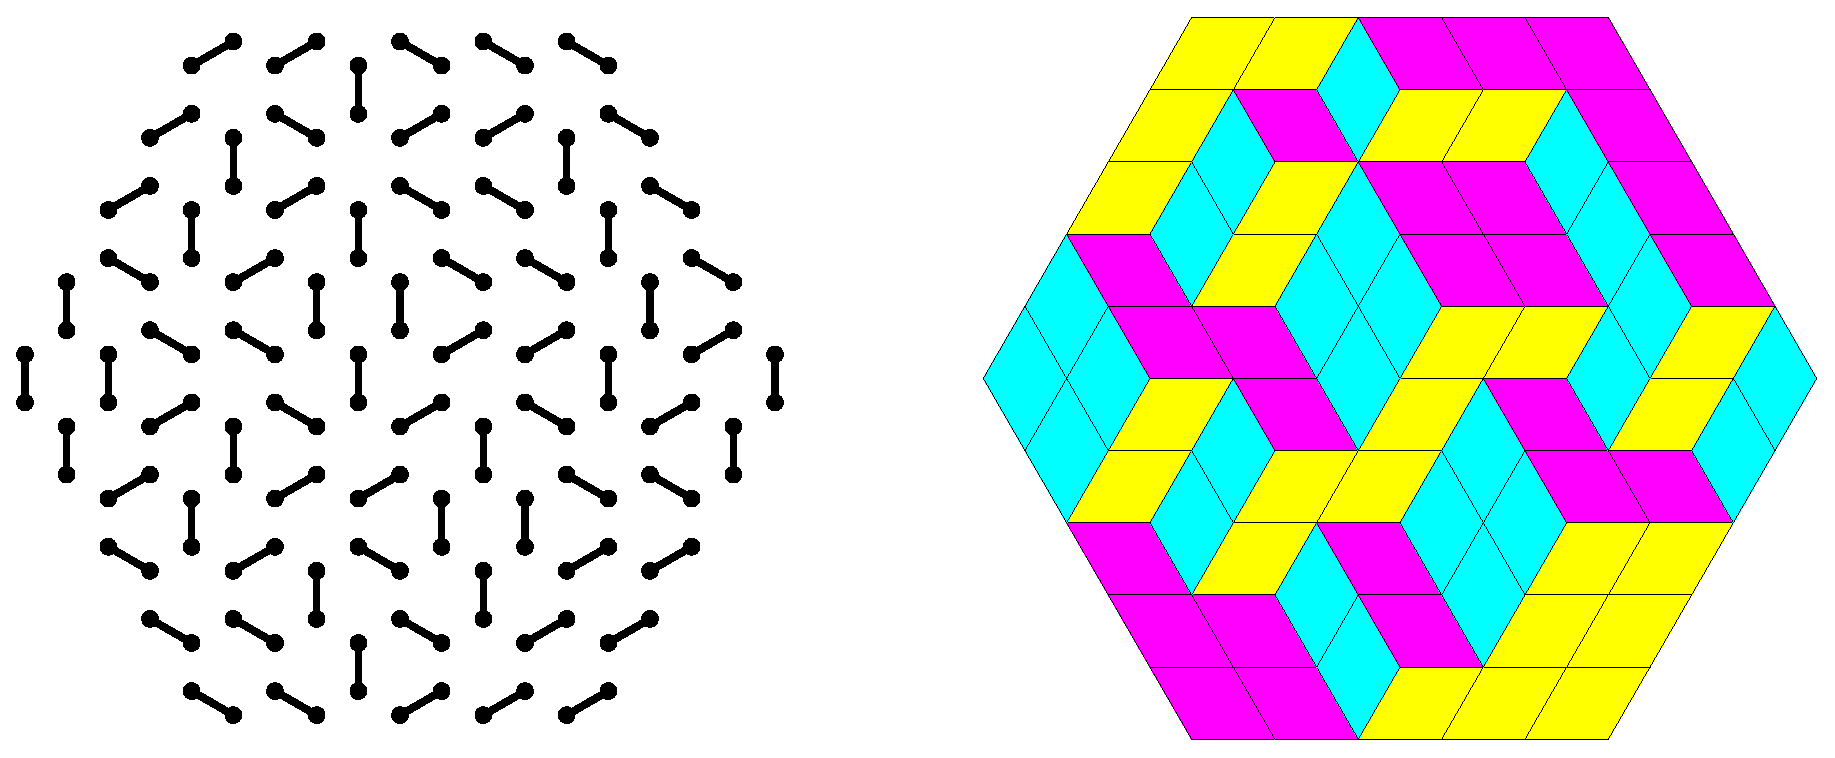
\includegraphics{loz.eps}}}
\caption{\label{dhf}A configuration of dimers on the hexagonal lattice and a corresponding picture
  of ``cubes in the corner''.}
\end{figure}

Let us define the sizes $M$, $N$, and $K$ of the sides of the hexagon.
The above description can be formalized by
%set of configurations of the model can be defined all possible ways to write
setting the non-negative numbers up to $K$ in the boxes of the rectangular $M\times N$ table so that a value in
each box is not greater than values in the adjacent upper and left boxes
\begin{equation}
  \label{eq:1}
  h_{ij}\leq h_{i-1,j},\quad h_{ij}\leq h_{i,j-1}.
\end{equation}

The weight of a particular configuration is given by the exponent of the volume of all cubes or by a
sum of the height function values:
\begin{equation*}
  \label{eq:10}
  E[conf]=\sum_{i,j} h_{ij}=\mathrm{Volume}
\end{equation*}
We set Boltzman constant equal to 1 and choose system of units in such a way that there is no
coupling constant in the expression for energy. Then the partition function is
\begin{equation*}
  \label{eq:14}
  Z=\sum_{conf} e^{-\frac{E[conf]}{T}}=\sum_{conf}q^{\mathrm{Volume}[conf]}, 
\end{equation*}
where $q=\exp\left(-1/T\right)$ .

For this particular case, the partition function is given by the classical Macmahon combinatorial
formula~\cite{vuletic2009generalization}
\begin{equation}
  \label{eq:12}
   Z[M,N,K,q]=\prod_{i=1}^{M}\prod_{j=1}^{N}\prod_{k=1}^{K}\frac{1-q^{i+j+k-1}}{1-q^{i+j+k-2}}
\end{equation}


MacMahon formula is obtained for the following definition of the Kasteleyn matrix. Embed the
hexagonal lattice in the complex plane $\mathbb{C}$ in such a way that some edges are parallel to
the real line with and corresponding vertices have coordinates with integer real and imaginary
parts. Then take
\begin{eqnarray}
  \label{eq:18}
  {\cal K}(w,b)=q^{\Re w+\Im w} \quad \mathrm{if}\quad \Im w=\Im b\\
  {\cal K}(w,b)=1 \quad \mathrm{if}\quad \Im w\neq\Im b
\end{eqnarray}


The   free energy per site is defined as$^{*}$
\footnote{For convenience we omit the factor $\frac{1}{T}$ in the usual definition of the free energy.}
\begin{equation*}
  \label{eq:17}
  % \frac{f}{T}
  f=-\frac{1}{V}\ln Z(M,N,K,q)
\end{equation*}
Here $V$ is the number of vertices, it is twice the number of dimers and twice the number of  cube faces:
\begin{equation}
  \label{eq:19}
  V=2(MN+NK+MK)=2(ab+bc+ca) \varepsilon^{-2}
\end{equation}

We are interested in the scaling limit, combined with the thermodynamic limit, when $ T\to \infty,$
and $M,N,K\to \infty$, such that ratios $\frac{M}{T}=a,\quad \frac{N}{T}=b, \quad \frac{K}{T}=c$
remain fixed. In what follows we use $\varepsilon=\frac{1}{T}$, which can be seen as the scale of
the model, e.g. mesh size due to our choice of the system of units.

In the next section we compute the asymptotic expansion of the free energy $f$ in $\varepsilon$ and
derive $\varepsilon$-independent closed expressions for the first several coefficients in this
expansion.
  
\section{The computation of the free energy asymptotic expansion}
\label{sec:free-energy-scaling}
First we substitute MacMahon formula \eqref{eq:12} into the free energy definition \eqref{eq:17} and
obtain
\begin{multline}
  \label{eq:20}
    %-\frac{f}{T}
    f=-\frac{1}{V}\ln Z =\\=- \sum_{i=1}^{M} \sum_{j=1}^{N} \sum_{k=1}^{K} \frac{1}{V}\left[
  \ln\left(1-e^{-\varepsilon (i+j+k-3)} e^{-2\varepsilon}\right) -\ln\left(1-e^{-\varepsilon
      (i+j+k-3)} e^{-\varepsilon}\right)\right] 
\end{multline}
We need to notice that for a finite $\varepsilon$ and each value of $i,j,k$ the logarithms have the
form $\ln(1-x)$, where $0<x<1$. Thus we can represent the logarithms as a power series of $x$ and
obtain
\begin{equation}
  \label{eq:7}
  f=-\sum_{i=1}^{M} \sum_{j=1}^{N} \sum_{k=1}^{K}\sum_{n=1}^{\infty}
  \frac{1}{V}\frac{1}{n}\left[-e^{-n\varepsilon (i+j+k-3)} e^{-2n\varepsilon}+e^{-n\varepsilon
      (i+j+k-3)} e^{-n\varepsilon}\right] 
\end{equation}
Here we have an absolutely convergent series, so we can change the order of summation and rewrite
the free energy as
\begin{equation}
  \label{eq:37}
  f=-\sum_{n=1}^{\infty}
  \frac{1}{V}\frac{1}{n}e^{-n\varepsilon}\left(1-e^{-n\varepsilon}\right)\sum_{i=1}^{M}
  \sum_{j=1}^{N} \sum_{k=1}^{K}e^{-n\varepsilon (i+j+k-3)} 
\end{equation}
The triple sum factorizes into the product of three sums of the type $\sum_{i=0}^{M-1}e^{-n\varepsilon
  i}$, that are just the
 sums of geometric progression. So we have $\sum_{i=0}^{M-1}e^{-n\varepsilon
  i}=\frac{1-e^{-Mn\varepsilon}}{1-e^{-n\varepsilon}}$, and obtain
\begin{equation}
  \label{eq:38}
  f=-\sum_{n=1}^{\infty}
  \frac{1}{V}\frac{1}{n}\frac{e^{-n\varepsilon}}{\left(1-e^{-n\varepsilon}\right)^{2}}
  \left(1-e^{-na}\right)\left(1-e^{-nb}\right)\left(1-e^{-nb}\right) 
\end{equation}
Denote by $\chi(z)$ the function
\begin{equation}
  \label{eq:39}
  \chi(z)=e^{-z}\left(\frac{z}{1-e^{-z}}\right)^{2}, 
\end{equation}
and by $H_{n}$ the product of $\varepsilon$-independent exponents
\begin{equation}
  \label{eq:40}
  H_{n}=\left(1-e^{-na}\right)\left(1-e^{-nb}\right)\left(1-e^{-nc}\right).
\end{equation}

The function $\chi(z)$ is smooth in 0, even and has the following Taylor series:
\begin{equation}
  \label{eq:45}
  \chi(z)=1 - \frac{z^2}{12} + \frac{z^4}{240}+\mathcal{O}(z^{6})
\end{equation}

Using the definition of the volume \eqref{eq:19} the free energy is written as
\begin{equation}
  \label{eq:41}
  f=-\frac{1}{2(ab+bc+ca)} \sum _{n=1}^{\infty} \frac{\chi(n\varepsilon)}{n^{3}} H_{n}
\end{equation}
We are interested in the scaling behavior in $\varepsilon$ when $\varepsilon\to 0$. The function $f$
is regular in $\varepsilon$ for $\varepsilon>0$. So we need to
compute  $\left.f\right|_{\varepsilon\to 0}$ and the derivatives $\left.\frac{\partial f}{\partial
  \varepsilon}\right|_{\varepsilon\to 0}$, $\left.\frac{\partial^{2} f}{\partial
  \varepsilon^{2}}\right|_{\varepsilon\to 0}$.

For $\left.f\right|_{\varepsilon\to 0}$ we have $\chi(0)=1$ and the sum $\sum_{n=1}^{\infty}
\frac{H_{n}}{n^{3}}$ is just a sum of  polylogarithms
$\mathrm{Li}_{s}(z)=\sum_{n=1}^{\infty}\frac{z^{n}}{n^{s}}$ of third order:
\begin{multline}
  \label{eq:42}
  \left.f\right|_{\varepsilon\to 0} =\frac{1}{2(ab+bc+ca)}\left[\Li_{3}(e^{-a})+\Li_{3}(e^{-b})+\Li_{3}(e^{-c})-
    \Li_{3}(e^{-a-b})\right.\\
  \left.-\Li_{3}(e^{-b-c})-    \Li_{3}(e^{-a-c})+    \Li_{3}(e^{-a-b-c})-\zeta(3)\right]
\end{multline}
Here Riemann zeta function appears as a particular value of polylogarithm $\Li_{3}(1)=\zeta(3)$.

The derivative of the function $\chi(z)$ is zero, $\chi'(0)=0$, and the series
$\sum_{n=1}^{\infty} \frac{\chi'(n\varepsilon)}{n^{2}}H_{n}$ are convergent for a finite
$\varepsilon$, thus we have for a derivative
\begin{equation}
  \label{eq:43}
\left.\frac{\partial f}{\partial \varepsilon}\right|_{\varepsilon\to 0}=0
\end{equation}

Now let us compute the second derivative
\begin{equation}
  \label{eq:44}
\frac{\partial^{2} f}{\partial
  \varepsilon^{2}}=-\frac{1}{2(ab+bc+ca)} \sum _{n=1}^{\infty} \frac{\chi''(n\varepsilon)}{n} H_{n}.  
\end{equation}
Second derivative of $\chi$ is finite $\chi''(0)=-\frac{1}{6}$. But there is a difficulty with the
limit $\varepsilon\to 0$ in this expression due to the poor convergence of the series. Let us
rewrite the second derivative as a sum of two series:
\begin{equation}
  \label{eq:46}
\frac{\partial^{2} f}{\partial
  \varepsilon^{2}}=-\frac{1}{2(ab+bc+ca)} \left(\sum _{n=1}^{\infty} \frac{\chi''(n\varepsilon)}{n}+
  \sum_{n=1}^{\infty} \frac{\chi''(n\varepsilon)}{n}(H_{n}-1)\right).    
\end{equation}
The second sum is now convergent, since $H_{n}-1$ decays exponentially in $n$. It can be presented
as a combination of series for logarithms:
\begin{multline}
  \label{eq:47}
  \chi''(0)\sum_{n=1}^{\infty} \frac{H_{n}-1}{n}=\\=\chi''(0)\sum_{n=1}^{\infty}\frac{1}{n}\left(-e^{-a
      n-b n-c n}+e^{-a n-b n}+e^{-a n-c n}+e^{-b n-c n} - e^{-a n}-e^{-b n}-e^{-c n}\right)=\\
  =\frac{1}{6}\ln\left(\frac{(e^{a}-1)(e^{b}-1)(e^{c}-1)(e^{a+b+c}-1)}{(e^{a+b}-1)(e^{b+c}-1)(e^{a+c}-1)}\right)
%%  =\frac{1}{6} \left(-\log \left(1-e^{-a-b-c}\right)+\log
%%   \left(1-e^{-a-b}\right)+\log
%%   \left(1-e^{-a-c}\right)+\log
%%   \left(1-e^{-b-c}\right)-\log
%%   \left(1-e^{-a}\right)-\log
%%   \left(1-e^{-b}\right)-\log
%%   \left(1-e^{-c}\right)\right)
\end{multline}

First sum in the expression \eqref{eq:46} can be expressed as follows. First, consider second
derivative of $\chi(z)$, separate an exponent and denote what is left by $\xi(z)$:
\begin{equation}
  \label{eq:48}
  \chi''(z)=e^{-z}\frac{e^{2 z} \left(z^2+4 e^z
   \left(z^2-1\right)+e^{2 z} \left(z^2-4
   z+2\right)+4
   z+2\right)}{\left(e^z-1\right)^4}=e^{-z}\xi(z)
\end{equation}
The sum is then rewritten
\begin{equation}
  \label{eq:49}
  \sum _{n=1}^{\infty} \frac{\chi''(n\varepsilon)}{n}=
  \sum_{n=1}^{\infty}\frac{e^{-n\varepsilon}}{n}\xi(n\varepsilon) =
  \sum_{n=1}^{\infty}\frac{e^{-n\varepsilon}}{n}\xi(0)+  \varepsilon\sum_{n=1}^{\infty}e^{-n\varepsilon}\frac{\xi(n\varepsilon)-\xi(0)}{n\varepsilon}   
\end{equation}
The first term is series for the logarithm $\ln\left(1-e^{-\varepsilon}\right)\approx \ln
\varepsilon$,
the second term can approximated by the integral:
\begin{equation}
  \label{eq:50}
  \varepsilon\sum_{n=1}^{\infty}e^{-n\varepsilon}\frac{\xi(n\varepsilon)-\xi(0)}{n\varepsilon}\approx
  \int_{0}^{\infty} e^{-z}\frac{\xi(z)-\xi(0)}{z} dz
\end{equation}
\begin{equation}
  \label{eq:51}
  \frac{\partial^{2} f}{\partial
  \varepsilon^{2}}\approx-\frac{1}{2(ab+bc+ca)}
\left[\frac{1}{6}\ln\left(\frac{(e^{a}-1)(e^{b}-1)(e^{c}-1)(e^{a+b+c}-1)}{(e^{a+b}-1)(e^{b+c}-1)(e^{a+c}-1)}\right)-\frac{1}{6}\ln \varepsilon+\int_{0}^{\infty} e^{-z}\frac{\xi(z)-\xi(0)}{z} dz\right]
\end{equation}
Since we have logarithmic term in the second derivative, we have the behavior of free energy of the form
\begin{equation}
  \label{eq:26}
  f\approx f_{0}+f_{1}\varepsilon +f_{2}\varepsilon^{2}\ln\varepsilon+ f_{3}\varepsilon^{2}+\mathcal{O}(\varepsilon^{3}),
\end{equation}
as expected in general in two-dimensional critical systems \cite{cardy1988finite}. Taking the
derivatives of such expression by $\varepsilon$, we get $f_{0}=f(0)$,
$f_{1}=\left.\frac{\partial f}{\partial \varepsilon}\right|_{\varepsilon\to 0}$,
$\frac{\partial^{2} f}{\partial \varepsilon^{2}}=f_{2}(2\ln\varepsilon+3)+f_{3}$. 

Thus we have the coefficients
\begin{multline}
  \label{eq:27}
  f_{0}=\frac{1}{2(ab+bc+ca)}\left[\Li_{3}(e^{-a})+\Li_{3}(e^{-b})+\Li_{3}(e^{-c})-
    \Li_{3}(e^{-a-b})\right.\\
  \left.-\Li_{3}(e^{-b-c})-    \Li_{3}(e^{-a-c})+    \Li_{3}(e^{-a-b-c})-\zeta(3)\right]
\end{multline}


\begin{equation}
  \label{eq:28}
  f_{1}=0,
\end{equation}
\begin{equation}
  \label{eq:30}
  f_{2}=-\frac{1}{2(ab+bc+ca)}\frac{1}{12},
\end{equation}
and
\begin{equation}
  \label{eq:29}
  f_{3}=-\frac{1}{2(ab+bc+ca)}\left[\frac{1}{12}\ln\left(\frac{(e^{a}-1)(e^{b}-1)(e^{c}-1)(e^{a+b+c}-1)}{(e^{a+b}-1)(e^{b+c}-1)(e^{a+c}-1)}\right)-\frac{1}{8}+ \frac{1}{2}\int_{0}^{\infty} e^{-z}\frac{\xi(z)-\xi(0)}{z} dz
    \right].
\end{equation}



\section{Physical meaning of the expansion coefficients}
\label{sec:accur-expans-phys}

In the paper \cite{1742-6596-1135-1-012024} we have presented results of Monte Carlo simulations using
Metropolis and Wang-Landau algorithms that support the form of expansion (\ref{eq:26}). In
particular we got $f_{1}=0.04\pm 0.04$ which is consistent with $f_{1}=0$. 

In the scaling limit $\varepsilon\to 0$ so called ``limit shape phenomenon''~\cite{1998math......1068J,cohn1998shape}
appears in the dimer model. The areas around the corners of the domain are ``frozen'' with height
function values being fixed. An analytical ``Arctic curve'' delimits frozen regions from the region
where the behavior is described by the effective free field theory
\cite{kenyon2009lectures,kenyon2008height,kenyon2006dimers}.

The behavior (\ref{eq:26}) of the logarithm of the partition function is generic in two-dimensional
models \cite{cardy1988finite}.

First two terms $f_{0}$ and $f_{1}$ are interpreted as a bulk and
boundary free energies in the corresponding field theory. Since we have $f_{1}=0$, we can conclude
that boundary tension is zero.
The value of the first term $f_{0}$ can be rewritten using polylogarithm functions as

The term proportional to the logarithm of the scale $\varepsilon$ is also universal
\cite{cardy1988finite} and should appear in all two-dimensional theories with boundary. In the paper
\cite{cardy1988finite} it was argued that on a manifold of a characteristic length $L$ with a smooth
boundary such a term must have the following form:
\begin{equation}
  \label{eq:31}
  \delta F = -\frac{1}{6}{\bf c} \chi \ln L,
\end{equation}
where ${\bf c}$ is central charge of the effective field theory and $\chi$ is the Euler characteristic of
the manifold
\begin{equation}
  \label{eq:32}
  \chi=2-2 h-b,
\end{equation}
where $h$ is the number of handles and $b$ is the number of boundaries. 

Since the non-frozen domain is delimited by a smooth boundary, we have $\chi=1$ and we interpret
$2(ab+bc+ca)$ as a volume of the domain, thus
\begin{equation}
  \label{eq:33}
  \delta F = \left(2(ab+bc+ca)\right) f_{2}\ln\varepsilon,
\end{equation}
which together with formula \eqref{eq:30} suggests the value of central charge
${\bf c}=\frac{1}{2}$. This value is in agreement with the identification of the dimer model with
free fermions in the paper \cite{dijkgraaf2009dimer}.

The last term $f_{3}$ depends only on the shape of the domain through $a,b,c$ with a universal
contribution that is equal to the integral of a function $e^{-z}\frac{\xi(z)-\xi(0)}{z}$. We conjecture
this constant will appear even for a different choice of Kasteleyn weighting, due to the treatment
of logarithmic divergency. In the future work we will consider coordinate dependent values of $q$
and more complex geometries, as was done in the paper \cite{okounkov2007random}, to check this
suggestion.

\section{Numeric checks}
\label{sec:numeric-checks}
To check our result \eqref{eq:26} numerically, we first need to evaluate the integral in $f_{3}$.
The function $e^{-z}\frac{\xi(z)-\xi(0)}{z}$ is smooth and but some care is required when taking the
limit $z\to 0$ numerically. Evaluating the integral numerically with Mathematica we get
\begin{equation}
  \label{eq:2}
  \int_{0}^{\infty}e^{-z}\frac{\xi(z)-\xi(0)}{z} dz = -0.08084228607897521
\end{equation}

The asymptotic expansion \eqref{eq:26} gives very good approximation for free energy. In Figure
\ref{fig:approx-acc} we present exact and approximate values for $f$ and, on the right panel,
demonstrate that inaccuracy is actually $\mathcal{O}(\varepsilon^{4})$. 

\begin{figure}[htbp]
  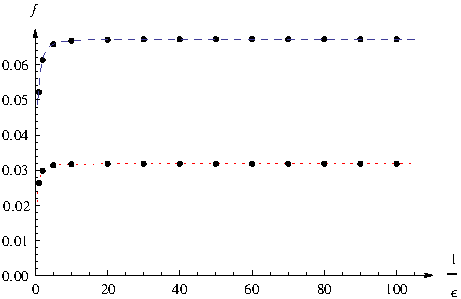
\includegraphics[scale=0.9]{exact-vs-approximation}
  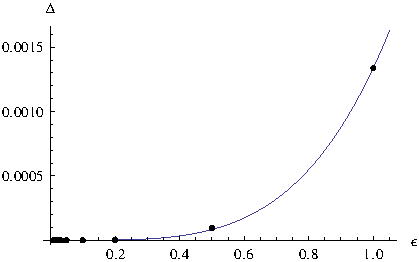
\includegraphics{error-1}
  \caption{\label{fig:approx-acc} {\it On the left:} Dependence of free energy on $1/\varepsilon$,
    top -- $a=b=c=1$, bottom -- $a=3, b=2, c=1$. Exact values are shown by solid dots.
    Approximations with formula \eqref{eq:26} are shown as blue dashed and red dotted lines. {\it On
      the right:} Dependence of approximation inaccuracy on $\varepsilon$, solid line is fit by $b\varepsilon^{4}$.}
\end{figure}

\section{Generalization to other domains and particular cases}
\label{sec:gener-other-doma}

Consider the case of cubes in the box of infinite height. In this case $K=\infty$ and $M,N$ are
finite. Now the hexagonal domain of dimer configurations has side of infinite length and total
number of dimers is infinite, so it is more natural to set the volume of the system $V=MN$.  

Putting $K=\infty$ in the partition function, we see that all terms with $k$ are cancelled and we have
\begin{equation}
  \label{eq:3}
  Z[M,N,q]=\prod_{i=1}^{M}\prod_{j=1}^{N}\frac{1}{1-q^{i+j-1}}
\end{equation}

The computation of free energy is almost exactly the same as in finite box case. We expand the
logarithm in the free energy and then factorize the sum:
\begin{multline}
  \label{eq:4}
  f=-\frac{1}{MN}\sum_{i=1}^{M}\sum_{j=1}^{N}\ln\left(1-e^{-\varepsilon(i+j-2)}e^{-\varepsilon}\right)=\\
  =\sum_{n=1}^{\infty}\frac{\varepsilon^{2}}{ab}\frac{1}{n}e^{-n\varepsilon}\left(\sum_{i=1}^{M}e^{-n\varepsilon(i-1)}\right)
  \left(\sum_{j=1}^{N}e^{-n\varepsilon(j-1)}\right)
\end{multline}
Computing the sums of geometric progressions we obtain almost the same expression as \eqref{eq:38},
except that $H_{n}$ now has two multipliers $H_{n} =\left(1-e^{-na}\right)\left(1-e^{-nb}\right)$:
\begin{equation}
  \label{eq:5}
  f=-\frac{1}{ab} \sum_{n=1}^{\infty}\frac{\chi(n\varepsilon)}{n^{3}} H_{n}.
\end{equation}
The function $\chi(z)=e^{-z}\left(\frac{z}{1-e^{-z}}\right)^{2}$ is the same as in \eqref{eq:39}.

Doing the same computations as in section \ref{sec:free-energy-scaling}, we obtain following results
for the coefficients $f_{0}, f_{1}, f_{2}, f_{3}$:
\begin{equation}
  \label{eq:6}
  f_{0}=\frac{1}{ab}\left[\Li_{3}(e^{-a})+\Li_{3}(e^{-b})-
    \Li_{3}(e^{-a-b})-\zeta(3)\right]
\end{equation}
\begin{equation}
  \label{eq:8}
  f_{0}=0
\end{equation}
\begin{equation}
  \label{eq:9}
  f_{2}=\frac{1}{ab}\frac{1}{12}
\end{equation}
\begin{equation}
  \label{eq:11}
  f_{3}=-\frac{1}{ab}\left[\frac{1}{12}\ln\left(\frac{(e^{a}-1)(e^{b}-1)}{(e^{a+b}-1)}\right)-\frac{1}{8}+ \frac{1}{2}\int_{0}^{\infty} e^{-z}\frac{\xi(z)-\xi(0)}{z} dz
    \right].
\end{equation}

Again in the Fig. \ref{fig:approx-acc-2d} we see good numerical agreement between the asymptotic
expansion \eqref{eq:26} and the exact formula \eqref{eq:4}.

\begin{figure}[htbp]
  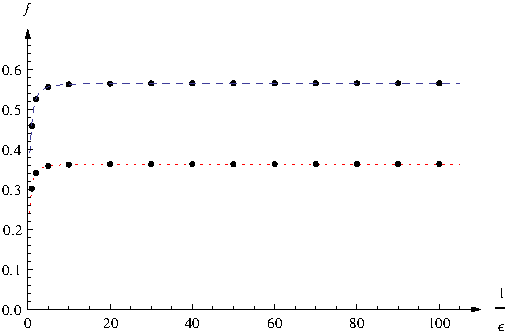
\includegraphics[scale=0.8]{exact-vs-approximation-2d}
  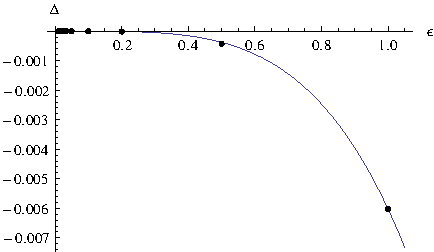
\includegraphics[scale=0.9]{error-2d}
  \caption{\label{fig:approx-acc-2d} {\it On the left:} Dependence of free energy on $1/\varepsilon$
    in the infinite height box,
    top -- $a=b=1$, bottom -- $a=2, b=1$. Exact values are shown by solid dots.
    Approximations with formula \eqref{eq:26} are shown as blue dashed and red dotted lines. {\it On
      the right:} Dependence of approximation inaccuracy on $\varepsilon$, solid line is fit by $b\varepsilon^{4}$.}
\end{figure}

Let us consider the generalization to the case when $q$ depends upon the coordinate. It's usually
done by varying $q$ on diagonal slices numbered by $t$. We need proper setup to consider the scaling
limit. Let $\varphi(t)$ be a continuous bounded smooth function for $t\in\left[-a,b\right]$. Denote by
$q_{i}=e^{-\varepsilon \varphi\left(i\varepsilon\right)}$ for $i=(-M+1)\dots N-1$. We index diagonal slices in
such a way, that top left corner of the $M\times N$ box has index $N-M$, top right corner -- $N$,
bottom left -- $-M$ and bottom right -- $0$. (See Fig. \ref{fig:box-t-coords} ). The slices with the
indexes $N$ and $-M$ are empty so we set $q_{N}=q_{-M}=0$. There can be at most $N+M-1$ non-empty
slices. 

\begin{figure}[htbp]
  \includegraphics[scale=0.5]{box-t-coords}
  \caption{\label{fig:box-t-coords} Coordinates of slices.}
\end{figure}

The partition function for this and more general case of arbitrary inner shape of the box was
presented in the paper \cite{okounkov2007random}. In this case it contains products of weights
$q_{i}$ for slices with negative and positive indexes:
\begin{equation}
  \label{eq:13}
  Z=\prod_{i=0}^{N-1}\prod_{j=0}^{M-1} \frac{1}{1-q_{N-M}^{-1}\left(\prod_{k=0}^{i}q_{N-M-k}\right)\left(\prod_{l=0}^{j}q_{N-M+l}\right)}
\end{equation}
(see Theorem 2 in \cite{okounkov2007random}).
If we set $q_{i}=q$, we recover formula \eqref{eq:3}.

Now let us again consider free energy dependence on $\varepsilon$:
\begin{equation}
  \label{eq:21}
  f=-\frac{\varepsilon^{2}}{ab}\sum_{i=0}^{N-1}\sum_{j=0}^{M-1}\ln
  \left(1-e^{\varepsilon \varphi(b-a)}e^{-\varepsilon\sum_{k=0}^{i}\varphi\left(b-a-k\varepsilon\right)}
    e^{-\varepsilon\sum_{l=0}^{j}\varphi\left(b-a+l\varepsilon\right)} \right)
\end{equation}
Expand the logarithm, change the order of summation and rewrite the free energy in the same way as
we did before:
\begin{equation}
  \label{eq:22}
   f=\sum_{n=1}^{\infty}\frac{\varepsilon^{2}}{ab}\frac{1}{n}e^{n\varepsilon
     \varphi(b-a)}\sum_{i=0}^{N-1}\sum_{j=0}^{M-1} e^{-n\varepsilon\sum_{k=0}^{i}\varphi\left(b-a-k\varepsilon\right)}
    e^{-n\varepsilon\sum_{l=0}^{j}\varphi\left(b-a+l\varepsilon\right)}
\end{equation}
Now we again can factorize double sum into product of two sums:
\begin{equation}
  \label{eq:23}
    f=\sum_{n=1}^{\infty}\frac{\varepsilon^{2}}{ab}\frac{1}{n}e^{-n\varepsilon
     \varphi(b-a)}\left(1+\sum_{i=1}^{N-1}
     e^{-n\varepsilon\sum_{k=1}^{i}\varphi\left(b-a-k\varepsilon\right)}\right)
   \left(1+\sum_{j=1}^{M-1}e^{-n\varepsilon\sum_{l=1}^{j}\varphi\left(b-a+l\varepsilon\right)}\right)
\end{equation}
Note that for $\varphi(t)\equiv 1$ we recover formula \eqref{eq:4}. 
%%  
%%  If we assume that $\varphi(b-a)\neq 0$, we can again obtain function $\chi(z)$:
%%  \begin{multline}
%%    \label{eq:24}
%%     f=\frac{1}{ab}\sum_{n=1}^{\infty}\frac{\chi\left(n\varepsilon\varphi(b-a)\right)}{n^{3}}\left(1-e^{-n\varepsilon
%%         \varphi(b-a)}\right)^{2}\frac{1}{\varphi^{2}(b-a)}\cdot\\
%%     \cdot\left(1+\sum_{i=1}^{N-1}
%%       e^{-n\varepsilon\sum_{k=1}^{i}\varphi\left(b-a-k\varepsilon\right)}\right)
%%     \left(1+\sum_{j=1}^{M-1}e^{-n\varepsilon\sum_{l=1}^{j}\varphi\left(b-a+l\varepsilon\right)}\right)  
%%  \end{multline}
%%

We need to separate contributions of different orders in $\varepsilon$ and keep only the terms up to
$\varepsilon^{2}$. To do so we expand the exponent
\begin{equation}
  \label{eq:35}
e^{-n\varepsilon\varphi(b-a)}\approx
1-n\varepsilon\varphi(b-a)+\frac{1}{2}n^{2}\varepsilon^{2}\varphi^{2}(b-a)+\mathcal{O}(\varepsilon^{3})  ,
\end{equation}
and approximate the sums by integrals using Euler-Maclaurin formula.

The sum $\varepsilon\sum_{k=1}^{i}\varphi\left(b-a-k\varepsilon\right)$ can be approximated using
Euler-Maclaurin formula:
\begin{multline}
  \label{eq:25}
  \varepsilon\sum_{k=1}^{i}\varphi\left(b-a-k\varepsilon\right)=\int_{0}^{i\varepsilon}\varphi(b-a-x)\dx
  +\frac{\varepsilon}{2}\left(\varphi(b-a)+\varphi(b-a-i\varepsilon)\right)+\\
  +\frac{1}{12}\varepsilon^{2}\left(\varphi'(b-a-i\varepsilon)-\varphi'(b-a)\right)+\mathcal{O}(\varepsilon^{3})
\end{multline}

Substituting into the exponent and expanding we get:
\begin{multline}
  \label{eq:34}
  e^{-n\varepsilon\sum_{k=1}^{i}\varphi\left(b-a-k\varepsilon\right)}\approx e^{-n\int_{0}^{i\varepsilon}\varphi(b-a-x)\dx
  -n\frac{\varepsilon}{2}\left(\varphi(b-a)+\varphi(b-a-i\varepsilon)\right)
  -n\frac{1}{12}\varepsilon^{2}\left(\varphi'(b-a-i\varepsilon)-\varphi'(b-a)\right)}\approx\\
\approx e^{-n\int_{0}^{i\varepsilon}\varphi(b-a-x)\dx}\left[1-\frac{n\varepsilon}{2}\left(\varphi(b-a)+\varphi(b-a-i\varepsilon)\right)+\right.\\\left.
  +\varepsilon^{2}\left(\frac{n^{2}}{8} \left(\varphi(b-a)+\varphi(b-a-i\varepsilon)\right)^{2}-\frac{n}{12}\left(\varphi'(b-a-i\varepsilon)-\varphi'(b-a)\right)\right)+\mathcal{O}(\varepsilon^{3})\right]
\end{multline}
Similarly, the expression for the second exponent is
\begin{multline}
  \label{eq:36}
 e^{-n\varepsilon\sum_{l=1}^{j}\varphi\left(b-a+l\varepsilon\right)}\approx e^{-n\int_{0}^{j\varepsilon}\varphi(b-a+x)\dx}\left[1-\frac{n\varepsilon}{2}\left(\varphi(b-a)+\varphi(b-a+j\varepsilon)\right)+\right.\\\left.
  +\varepsilon^{2}\left(\frac{n^{2}}{8} \left(\varphi(b-a)+\varphi(b-a+j\varepsilon)\right)^{2}-\frac{n}{12}\left(\varphi'(b-a+j\varepsilon)-\varphi'(b-a)\right)\right)+\mathcal{O}(\varepsilon^{3})\right]  
\end{multline}

Now we need to substitute this expansion and formula \eqref{eq:35} into our formula for free energy
\eqref{eq:23}. 


\section*{Conclusion and outlook}
\label{sec:conclusion}

In the present paper we computed the asymptotic expansion of the free energy in the dimer model on a
hexagonal domain of the hexagonal lattice. We've discussed the physical meaning of the expansion
coefficients and argued that our results support the identification of the scaling behavior of the
dimer model with the free-fermion field theory.

In further work we will show the connection of the expansion coefficients with the spectral
properties of Dirac operator on the non-frozen domain and study the universality of the presented
expressions by considering the model on more generic domain geometries with the non-uniform
Kasteleyn weighting with $q$ depending on the coordinate.

\section*{Acknowledgments}
\label{sec:acknowledgements}
I am grateful to professor Nikolai Reshetikhin for his guidance in this work. I thank Pavel Belov
for useful discussions and general support.

I thank the organizers and participants of the conference MQFT-2018 for the opportunity
to present our results and useful discussions.

This research is supported by RFBR grant No. 18-01-00916.

\bibliographystyle{utphys}
\bibliography{listing,bibliography,dimers}{} 
\end{document}
